\documentclass[]{report}
\usepackage[hmargin=1.25in,vmargin=1in]{geometry} %调整页边距
% \usepackage[inner=1in,outer=1.25in]{geometry} %书籍左右不等宽排版
\usepackage[utf8]{inputenc}
\usepackage[]{ctex} %据说可以直接调用诸如 \kaishu \fangsong \heiti 的命令修改字体
\usepackage[svgnames]{xcolor} % Using colors
% \usepackage{background} % To include background images
\usepackage{fancyhdr} % Needed to define custom headers/footers
\usepackage[]{xeCJK}
\setCJKmainfont[BoldFont = STHeiti, ItalicFont = STKaiti]{Songti SC Light} %中文主字体
\setCJKsansfont[BoldFont = Weibei SC, ItalicFont = HanziPen SC]{Xingkai SC Light} %中文无衬线字体
\setCJKmonofont[BoldFont = Libian SC, ItalicFont = STFangsong]{Yuanti SC Light} %中文等宽字体
\setmainfont{Times New Roman} %\rmfamily
\setsansfont[ItalicFont = American Typewriter]{Comic Sans MS} %\sffamily
\setmonofont{Courier} %\ttfamily
\newfontfamily\monaco{Courier}
\usepackage{titlesec}
\titleformat{\chapter}{\centering\huge\bfseries}{第~\thechapter~章}{1em}{}

\usepackage{ulem} %解决下划线、删除线之类的
\usepackage{listings}
\lstset{
language=C++,
numberstyle = \monaco\color[HTML]{FFD700},
basicstyle = \monaco,
keywordstyle = \color{blue}\bfseries,
commentstyle=\color[HTML]{006400}, %DarkGreen
tabsize = 4,
%backgroundcolor=\color{bg}
emph = {int,float,double,char,void},emphstyle=\color[HTML]{800080}, % Purple
emph ={[2]const, typedef},emphstyle = {[2]\color[HTML]{4682B4}} %SteelBlue
}

\usepackage{amsmath} %数学公式问题
\usepackage{amsthm} %公式环境,如proof
\usepackage{booktabs} %三线表
\newcommand{\tabincell}[2]{\begin{tabular}{@{}#1@{}}#2\end{tabular}} %解决单元格内部换行的问题
% 比如这个 Beijing & 0,5 & 1,6 & 2,7 & 3,8 & 4,9 & The number changes every 3 months \\
% 改成这个 \tabincell{l}{Beijing}& \tabincell{c}{0,5}& \tabincell{c}{1,6}& \tabincell{c}{2,7}& \tabincell{c}{3,8}& \tabincell{c}{4,9}& \tabincell{c}{The number changes \\ every 3 months} \\
% 一个单元格过长,整行都需要修改
% 可以配合 \resizebox*{h-width}{v-width}{contents, e.g.tabular} 使用

\usepackage{mathrsfs} %在公式里面使用那个最花的字体
\usepackage{amssymb} %公式里面用空心黑体和旧式字体
\usepackage{amssymb} %AMS符号
\usepackage{amsthm} %AMS定理环境

\usepackage{markdown} %使用markdown语法,在编译时需要打开 shell-escape 标记,即 $ xelatex --shell-escape example.tex
\markdownSetup{hashEnumerators = true} %允许使用 #. 的方式编写有序列表
\markdownSetup{inlineFootnotes = true} %允许使用脚注形式的超链接,调用语法为 [anchor](uri), ^[footnote], <uri>
\markdownSetup{fencedCode = true} %以反引号和缩进来插入代码段,相当于 verbatim
\markdownSetup{
  pipeTables = true
} %支持表格的用法 (图片已经在markdown包里面支持了)
% \usepackage{booktabs} %解决三线表的线条粗细问题

\usepackage{graphicx} %插入图片
\usepackage{pdfpages} %插入PDF文件
\usepackage{makeidx}

\usepackage{tikz} %带圈字符
\usepackage{etoolbox} %带圈字符 (提供robustify)
\usepackage{enumitem}
\newcommand*{\circled}[1]{\lower.7ex\hbox{\tikz\draw (0pt, 0pt)%
    circle (.5em) node {\makebox[1em][c]{\small #1}};}} %新定义命令:带圈字符
\robustify{\circled}
% \usepackage{enumerate} %有序列表

\usepackage{hyperref} %超链接
% \usepackage[hidelinks]{hyperref} %隐藏超链接的红框
\markdownSetup{
  inlineFootnotes = true,
  renderers = {
    link = {\href{#3}{#1}},
  }
} % markdown块中使用直接点进去的超链接
% \setlist[enumerate,1]{label=(\arabic*).,font=\textup,leftmargin=7mm,labelsep=1.5mm,topsep=0mm,itemsep=-0.8mm}
% \setlist[enumerate,2]{label=(\alph*).,font=\textup,leftmargin=7mm,labelsep=1.5mm,topsep=-0.8mm,itemsep=-0.8mm}

\usepackage{braket}

%%%%%% Setting up the style

% \setlength\parindent{0pt} % Gets rid of all indentation
% \backgroundsetup{contents={\includegraphics[width=\textwidth]{ustc-name.pdf}},scale=0.4,placement=top,opacity=0.6,color=cyan,vshift=-20pt} %  USTC Logo

\pagestyle{fancy} % Enables the custom headers/footers

% \lhead{n体问题实验报告} \rhead{N Body Problem} % Headers - all  empty

% \title{\vspace{-1.8cm}  \color{DarkRed} Laboratory Rotation Report}
% \subtitle{Title of the proposal % Title of the rotation project
% \vspace{-2cm} }
% \date{\today} % No date

\lfoot{\color{Grey} 艾语晨}  % Write your name here
\rfoot{ \color{Grey} N体问题 }
\cfoot{\color{Grey} \thepage}

\renewcommand{\headrulewidth}{0.0pt} % No header rule
\renewcommand{\footrulewidth}{0.4pt} % Thin footer rule

\linespread{1.3} %行间距为1.3倍默认间距 (1.3 x 1.2倍字符宽度)

\title{N体问题实验报告}
\author{艾语晨~PB18000227}
\date{\today}

\makeindex

\begin{document}
\theoremstyle{definition} \newtheorem{theorem}{Thm}[section] %定义一个定理Thm,序号为section的下一级序号
\theoremstyle{definition} \newtheorem{definition}{Def}[section] %定义一个定义Def,序号为section的下一级序号
\theoremstyle{plain} \newtheorem{lemma}{lemma}[section] %引理

	\maketitle
	\newpage

	\tableofcontents
	\newpage

	\chapter{背景介绍}
		在物理学中,n体问题是预测一组由万有引力相互吸引的天体的运动轨迹的问题。一直以来,了解日月星辰的运动成为解决此问题的动机。在20世纪,了解球状星团的动力学成了最为重要的n体问题。广义相对论中的n体问题很难解决。\par
		经典的物理问题可以非正式的表达为:
		\begin{quote}
			给定一组天体的准稳态轨道性质(瞬时位置,速度和时间),预测其相互作用力; 因此,可以预测未来所有时间的真实轨道运动。\footnote{以上译自Wikipedia}
		\end{quote}
		将各个星体抽象为质点,并根据经典力学的相关理论,若在三维空间中给定位置向量与各自的初速度向量,根据万有引力定律与Newton运动定律,可以计算出物体下一步的运动情况。为进一步简化问题,可以将时间分割为单位时间单元,以离散的时间变量代替连续的变量。

		\newpage
	\chapter{实验目的}
		成功安装Python 3.8、pygame并运行现有代码,并对其进行一定的改编,使之具有更多的功能,一个交互式界面

		\newpage
	\chapter{实验环境}
	\section{开发环境}
		本实验所用程序设计语言为python,版本为python-3.8.5。所用包管理工具为pip,版本为pip-20.2.1。
	\section{运行环境}
		本实验运行在Windows 10专业版操作系统(Mac虚拟机)上
	\section{工具}
		程序设计平台使用Visual Studio Code,运行代码使用 vscode 的插件 code runner
	\section{库}
		所用到的库函数如下:
		\begin{table}[h]
			\centering
			\caption{实验所用到的库文件}
			\begin{tabular}{c|c}
				\toprule
				MODULE&DESCRIPTION\\
				\midrule
				\verb|pygame|&GUI correlated\\
				\verb|stdio.py|&functions to read/write numbers and text from/to stdin and stdout\\
				\verb|stddraw.py|&functions to draw geometric shapes\\
				\verb|stdaudio.py|&functions to create, play, and manipulate sound\\
				\verb|stdrandom.py|&functions related to random numbers\\
				\verb|stdarray.py|&functions to create, read, and write 1D and 2D arrays\\
				\verb|stdstats.py|&functions to compute and plot statistics\\
				\verb|color.py|&data type for colors\\
				\verb|picture.py|&data type to process digital images\\
				\verb|instream.py|&data type to read numbers and text from files and URLs\\
				\verb|outstream.py|&data type to write numbers and text to files\\
				\bottomrule
			\end{tabular}
		\end{table}

		\newpage
	\chapter{实验内容}
	\section{原始代码}
		原有代码的设计是典型的封装和实例化的过程,其物理思想就是利用了牛顿万有引力定律,在微元近似的条件下,认为$\Delta t$时间内速度不变,通过$\vec{r'}=\vec{r}+\vec{v}\Delta t$计算出星体质点单位时间之后的坐标向量。人为建立一个坐标系并以向量来表示质点的参量,会简化计算。
	\section{改编部分}
		\subsection{设计概述}
		把4个N体问题文件组织在一个统一的文件里面,提供一个类似游戏的小程序。新的程序包括一个作者页、登陆界面(需要密码)和N体问题程序唤起页。
		\subsection{所用知识}
		利用Tkinter库的相关应用,如下:
		\begin{table}[h]
			\centering
			\begin{tabular}{ccc}
				\toprule
				类/方法&作用&使用位置\\
				\midrule
				\verb|tkinter.messagebox|&弹出消息框&登陆输入密码位置\\
				\verb|tkinter.font|&自定义字体&N体问题程序选择按钮\\
				\verb|tkinter.Label|&标签,显示文本或图像&密码输入提示文字、登陆页背景图片\\
				\tabincell{c}{\texttt{tkinter.Button}}&\tabincell{c}{按钮}&\tabincell{c}{结合事件响应弹出登陆密码输入框\\和带命令行参数运行N体问题程序}\\
				\verb|tkinter.Entry|&文本框&用于输入密码并显示为*\\
				\verb|tkinter.Canvas|&画布&用于放置Author Page\\
				\bottomrule
			\end{tabular}
		\end{table}
	\section{代码解析}
		\subsection{固定大小的窗口及自定义字体} 固定大小是为了和登陆界面的背景图片保持大小一致,而不是一开始展示的作者页;自定义字体改变了字体和字号,使得按钮上的文字更大更清楚。\par
		字符串中的空格在\LaTeX Listing中将显示为\begin{lstlisting}[language=python]
			' '
		\end{lstlisting},故我用下划线代替
		\begin{table}[h]
			\centering
			\begin{lstlisting}[language=python, basicstyle=\monaco]
root = tkinter.Tk(className='N_Body_Problem')
root.geometry('499x737')

# define my font
myFontHelvetica = font.Font(family='Helvetica', size=18, weight='bold')
			\end{lstlisting}
		\end{table}
		\subsection{作者页和登陆页} 作者页采用画布Canvas绘制,并调用 \verb|bind()| 函数,在鼠标左键抬起的时候响应,切换到登陆界面。登陆页采用Label定义其背景图片,有一个按钮,其绑定响应为登陆Messangbox弹窗,只有当输入密码为`lapland'时,登陆通过,调用 \verb|place_forget()| 隐藏登陆界面并创建4个按钮
		\paragraph{作者页} Author Page在Canvas上制作,定义 \verb|self.canvas| 实例,调用参数函数定义大小与背景颜色;调用tkinter的图片引入函数,将背景图片作为实例变量并导入画布;利用继承的canvas方法创建文字。此部分代码如下所示:
		\begin{lstlisting}[language=python, basicstyle=\monaco]
def ShowAuthor(self):
	self.canvas = tkinter.Canvas(self)
	self.canvas["width"] = 500
	self.canvas["height"] = 480
	self.canvas["bg"] = 'Azure'

	# import logo
	self.logo = tkinter.PhotoImage(file='phoenix6.png')
	self.canvas.create_image(250, 300, image=self.logo)

	# caption
	self.canvas.create_text(
		250, 80, font=myFontHelvetica, text="N_Body_Problem")
	self.canvas.create_text(
		250, 120, font=myFontHelvetica, text='by_OrigamiAyc')
	self.canvas.pack()

	# respond to Left-Click, changing to Author Page from Welcome Page
	self.canvas.bind('<ButtonRelease-1>', self.create_background)
		\end{lstlisting}
		\paragraph{登陆页} Login Page采取了与作者页不同的处理方式,即将Label组件作为背景嵌入到窗口的最底层,并在上层添加其他组件(这里为Button)。作者页与登陆页之间的跳转采用事件响应的策略,通过响应鼠标左键的抬起来跳转(上面的 \verb|self.canvas.bind()|)。按钮背景通过HTML5的十六进制RGB方式来赋值,按钮与背景标签均采用更灵活的 \verb|place()| 函数来相对于窗口定位。登陆操作通过弹窗输入密码来完成,调用使用messagebox的类MyDialog实例化一个password弹窗实例。通过MyDialog的成员方法 \verb|top()| 来等待弹窗结果,并调用方法 \verb|get()| 来接收返回值。在一个简单的 \verb|if| 语句判断之后,确定是否通过验证,并调用 \verb|showinfo()| 方法来报告给用户。此部分代码如下:
		\begin{lstlisting}[language=python, basicstyle=\monaco]
def create_background(self, events):
	self.canvas.pack_forget()
	self.backgroundname = tkinter.PhotoImage(file="ThreeBodyWelcome.png")
	self.background_label = Label(self.master, image=self.backgroundname)
	self.background_label.place(relx=0, rely=0)

	# Create a Button to Login
	# self.ThreeBodyLogin = tkinter.PhotoImage('ThreeBodyLogin.jpg')
	self.login = tkinter.Button(
		self.master, text='Login', command=self.Create_Message_Box)
	self.login['bg'] = '#87CEFA'  # DeepSkyBlue
	self.login.place(relx=0.46, rely=0.6)

def Create_Message_Box(self):
	password = MyDialog(self.master)
	self.login.wait_window(password.top)
	if password.get() == 'lapland':
		tkinter.messagebox.showinfo(
			'NBody', 'Welcome_to_the_world_of_NBody')
		self.create_buttons()
	else:
		tkinter.messagebox.showinfo('NBody', 'Incorrect_Password')
		\end{lstlisting}
		\paragraph{对话框} 对话框调用的类如下,定义了一个弹出式对话框并返回接收到的字符串的功能。
		\begin{lstlisting}[language=python, basicstyle=\monaco]
class MyDialog:
	def __init__(self, root):
		self.top = tkinter.Toplevel(root)
		label = tkinter.Label(self.top, text='Your_Password')
		label.pack()
		self.entry = tkinter.Entry(self.top, show='*')
		self.entry.pack()
		self.entry.focus()
		button = tkinter.Button(self.top, text='Ok',
								command=self.Ok)
		button.pack()

	def Ok(self):
		self.input = self.entry.get()
		self.top.destroy()

	def get(self):
		return self.input
		\end{lstlisting}
		\subsection{N体问题程序}
		在按钮页面上,四个按钮分别绑定在输入命令行参数运行Universe.py的方法上。这个方法实际上是对Universe.py里面的main函数加以改编得到的,即把命令提示符传参替换为方法调用传参。在命令行参数的传递方面,采用了三种思路:
		\begin{enumerate}
			\item 直接将命令行参数写在调用方法里面,作为其成员变量直接传入被调方法
			\item 使用lambda表达式
			\item 利用 \verb|functools| 包里面的 \verb|partial| 类,实例化一个中间参量作为关键字command的value
		\end{enumerate}\par
		此部分代码如下:
		\begin{lstlisting}[language=python, basicstyle=\monaco]
	def create_buttons(self):
		self.background_label.place_forget()
		self.login.place_forget()

		self.TwoBodyTiny = tkinter.Button(self)
		self.TwoBodyTiny["text"] = "TwoBodyTiny"
		self.TwoBodyTiny["command"] = self.TwoBodyTiny
		self.TwoBodyTiny['font'] = myFontHelvetica
		self.TwoBodyTiny['bg'] = '#98FB98'
		self.TwoBodyTiny['fg'] = '#800000'
		self.TwoBodyTiny['height'] = 1
		self.TwoBodyTiny['width'] = 15
		self.TwoBodyTiny['command'] = self.execTwoTiny
		self.TwoBodyTiny.pack(side=tkinter.TOP)

		self.TwoBody = tkinter.Button(self)
		self.TwoBody["text"] = "TwoBody"
		self.TwoBody["command"] = self.TwoBody
		self.TwoBody['font'] = myFontHelvetica
		self.TwoBody['bg'] = '#87CEFA'
		self.TwoBody['fg'] = '#8B008B'
		self.TwoBody['width'] = 15
		self.TwoBody['height'] = 1
		self.TwoBody['command'] = self.execTwoBody
		self.TwoBody.pack(side=tkinter.TOP)

		self.ThreeBody = tkinter.Button(self)
		self.ThreeBody["text"] = "ThreeBody"
		self.ThreeBody["command"] = self.ThreeBody
		self.ThreeBody['font'] = myFontHelvetica
		self.ThreeBody['bg'] = '#DEB887'
		self.ThreeBody['fg'] = '#191970'
		self.ThreeBody['height'] = 1
		self.ThreeBody['width'] = 15
		self.ThreeBody['command'] = lambda: self.execNBody(
			'3body.txt', 20000, stddraw.MAGENTA)
		self.ThreeBody.pack(side=tkinter.TOP)

		self.FourBody = tkinter.Button(self)
		self.FourBody["text"] = "FourBody"
		self.FourBody["command"] = self.FourBody
		self.FourBody['font'] = myFontHelvetica
		self.FourBody['bg'] = '#FFDEAD'
		self.FourBody['fg'] = '#228B22'
		self.FourBody['height'] = 1
		self.FourBody['width'] = 15
		self.FourExec = partial(
			self.execNBody, '4body.txt', 20000, stddraw.ORANGE)
		self.FourBody['command'] = self.FourExec
		self.FourBody.pack(side=tkinter.TOP)

	def execTwoTiny(self):
		filename = '2bodytiny.txt'
		dt = float(20000)
		PenColorTiny = stddraw.DARK_RED
		universe = Universe(filename)
		while True:
			universe.increaseTime(dt)
			stddraw.clear()
			universe.draw(PenColorTiny)
			stddraw.show(10)

	def execTwoBody(self):
		filename = '2body.txt'
		dt = float(20000)
		PenColor = stddraw.DARK_GREEN
		universe = Universe(filename)
		while True:
			universe.increaseTime(dt)
			stddraw.clear()
			universe.draw(PenColor)
			stddraw.show(10)

	def execNBody(self, fileName, calcFrequent, PenColor):
		self.filename = fileName
		self.dt = calcFrequent
		self.PenColor = PenColor
		self.universe = Universe(self.filename)
		while True:
			self.universe.increaseTime(self.dt)
			stddraw.clear()
			self.universe.draw(self.PenColor)
			stddraw.show(10)
		\end{lstlisting}
		\subsection{更改球体颜色}
		调用 \verb|stddraw.py| 库的方法 \verb|setPenColor()|,即可在 \verb|Body.py| 中修改所有的球体的颜色(同时修改)。为了设定自定义颜色,需修改 \verb|Body.py| 中 \verb|Body.draw()| 方法,以及 \verb|universe.py| 中 \verb|draw(), main()| 的对应接口参数。对应代码如下:
		\begin{lstlisting}[language=python, basicstyle=\monaco]
# in body.py
def draw(self, ColorSet=stddraw._DEFAULT_PEN_COLOR):
	stddraw.setPenRadius(0.0125)
	stddraw.setPenColor(ColorSet)
	stddraw.point(self._r[0], self._r[1])

# in universe.py
def draw(self, ColorSet):
	for body in self._bodies:
		body.draw(ColorSet)
		\end{lstlisting}

	\chapter{实验结果}
		下面放上运行截图,视频随压缩包附上
		\begin{figure}[h]
			\centering
			\begin{minipage}{40em}
				\begin{minipage}{18em}
					\centering
					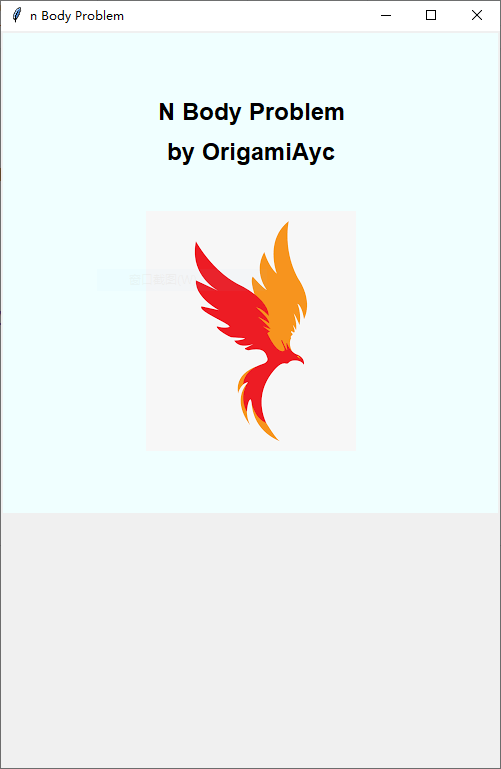
\includegraphics[scale=0.5]{pics/AuthorPage.PNG}
					\caption{Author Page}
				\end{minipage}
				\quad
				\begin{minipage}{18em}
					\centering
					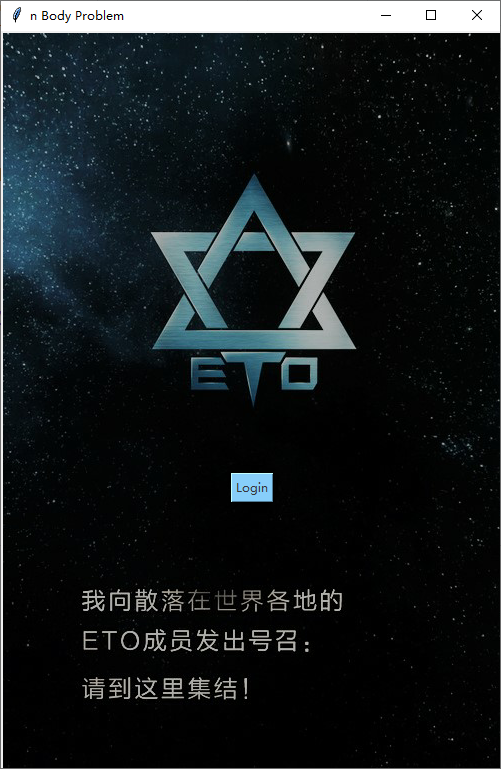
\includegraphics[scale=0.5]{pics/LoginPage.PNG}
					\caption{Login Page}
				\end{minipage}
			\end{minipage}
			\\[5pt]
			\begin{minipage}{40em}
				\centering
				\begin{minipage}{18em}
					\centering
					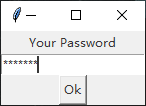
\includegraphics{pics/Password.PNG}
					\caption{Password Entering}
				\end{minipage}
				\quad
				\begin{minipage}{18em}
					\centering
					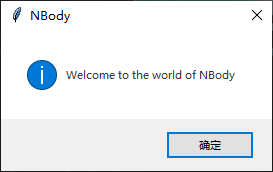
\includegraphics[scale=0.7]{pics/Verifyed.PNG}
					\caption{Password Verified}
				\end{minipage}
			\end{minipage}
		\end{figure}
		\begin{figure}[h]
			\centering
			\begin{minipage}{18em}
				\centering
				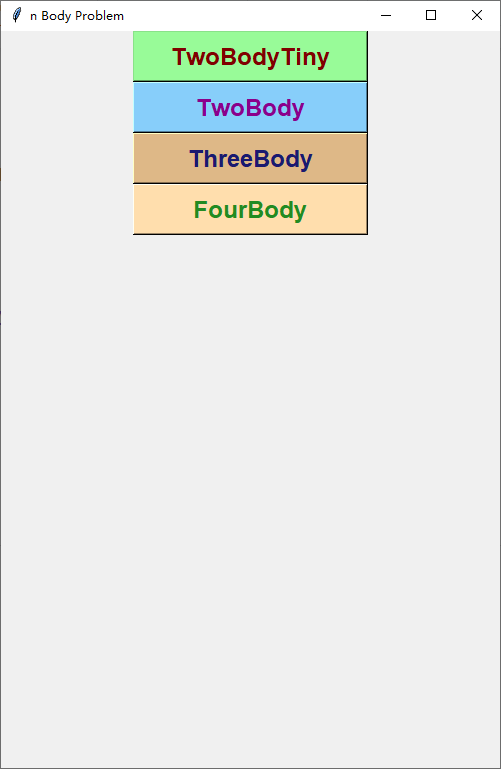
\includegraphics[scale=0.5]{pics/Buttons.PNG}
				\caption{Buttons}
			\end{minipage}
			\quad
			\begin{minipage}{18em}
				\centering
				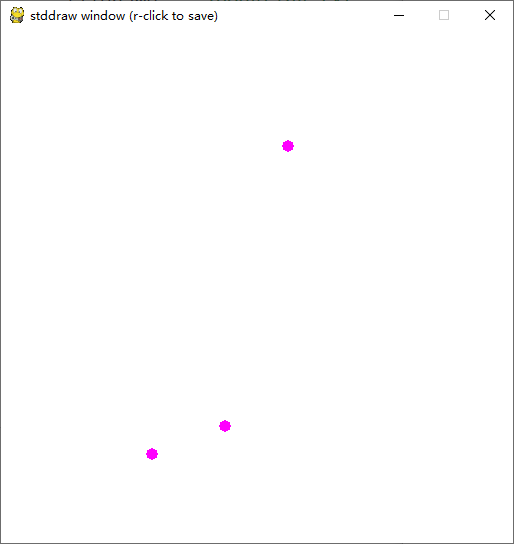
\includegraphics[scale=0.48]{pics/ThreeBody.PNG}
				\caption{ThreeBody Result}
			\end{minipage}
		\end{figure}

	\chapter{总结与收获}
		\begin{enumerate}
			\item 对于Tkinter库的使用有了很多了解,可以自己设计并完成一个简单的有交互界面窗口的应用
			\item 在复制粘贴代码的过程中对类的封装有了一些认识,可以通过封装类加上传递参数赋值的方式代替直接复制修改。可以增强代码可读性、增加简洁性、易于修改,类似于宏定义常参数的作用
			\item python入门,部分脱离C语言面向过程和涉及底层的影响(比如当我想开多线程的时候就不能直接系统调用)
		\end{enumerate}

	\chapter{参考资料及文献}
		\begin{enumerate}
			\item 《21天学通python 第二版》
			\item \textit{Learing Tkinter}
		\end{enumerate}

\end{document}
